\documentclass[a4paper,11pt, notitlepage, twosides, openany ]{report}
\usepackage[T1]{fontenc}
\usepackage[polish]{babel}
\usepackage[utf8]{inputenc}
\usepackage{lmodern}
\usepackage{enumitem}
\usepackage{indentfirst}
\usepackage{graphicx}
\usepackage{subcaption}
\usepackage{wrapfig}
\usepackage{fancyhdr}
\usepackage{lastpage}
\usepackage{listings}
\usepackage{spverbatim}
\usepackage{geometry}
\usepackage{amsmath,xparse}
\usepackage{listings}
\usepackage{color}
% \usepackage{amsfonts}
% \usepackage{amssymb}

\usepackage{url}
\usepackage{hyperref}

\pagestyle{fancy}
\fancyhf{}
\rfoot{Strona \thepage  \hspace{1pt} z \pageref{LastPage}}
\lhead{Projekt dyplomowy}

\hypersetup{
	colorlinks=true,
	linkcolor=black,
	filecolor=magenta,      
	urlcolor=black,
	citecolor=blue
}

\begin{document}
	
	\begin{titlepage}
		
		\newcommand{\HRule}{\rule{\linewidth}{0.5mm}} % Defines a new command for the horizontal lines, change thickness here
		
		\center % Center everything on the page
		
		%----------------------------------------------------------------------------------------
		%	HEADING SECTIONS
		%----------------------------------------------------------------------------------------
		
		\textsc{\LARGE Politechnika Warszawska}\\[1.5cm] % Name of your university/college
		\textsc{\Large Wydział Elektryczny }\\[0.5cm] % Major heading such as course name
		\textsc{\large Informatyka Stosowana }\\[1.0cm] % Minor heading such as course title
		
		%----------------------------------------------------------------------------------------
		%	TITLE SECTION
		%----------------------------------------------------------------------------------------
		
		% \HRule \\[0.4cm]
		{ \huge Wykrywanie współwystępowania obiektów\\ na obrazach cyfrowych}\\[2.0cm] % Title of your document
		% \HRule \\[1.5cm]
		
		%----------------------------------------------------------------------------------------
		%	AUTHOR SECTION
		%----------------------------------------------------------------------------------------
		
		\begin{minipage}{0.4\textwidth}
			\begin{flushleft} \large
				\emph{Wykonał:}\\
				 % Your name
			    Jakub \textsc{Korczakowski}\\
			\end{flushleft}
		\end{minipage}
		~
		\begin{minipage}{0.4\textwidth}
			\begin{flushright} \large
				\emph{Sprawdzający:} \\
				dr inż. Grzegorz \textsc{Sarwas} % Supervisor's Name
			\end{flushright}
		\end{minipage}\\[2cm]
		
		% If you don't want a supervisor, uncomment the two lines below and remove the section above
		%\Large \emph{Author:}\\
		%John \textsc{Smith}\\[3cm] % Your name
		
		%----------------------------------------------------------------------------------------
		%	DATE SECTION
		%----------------------------------------------------------------------------------------
		
		{\large \today}\\[2cm] % Date, change the \today to a set date if you want to be precise
		
		%----------------------------------------------------------------------------------------
		%	LOGO SECTION
		%----------------------------------------------------------------------------------------
		
		
\includegraphics[width = 28mm]{logo.jpg} % Include a department/university logo - this will require the graphicx package
		
		%----------------------------------------------------------------------------------------
		
		\vfill % Fill the rest of the page with whitespace
		
	\end{titlepage}
	\tableofcontents
	\newpage
	
	
	\chapter{Wstęp}
	Tematem mojej pracy dyplomowej jest \textit{Wykrywanie współwystępowania obiektów na obrazach cyfrowych}. Zadanie wykrywania współwystępowania obiektów (\textit{co-saliency detection}) polega na wyszukiwaniu na obrazach cyfrowych obszarów istotnych oraz częstych \cite{10.1145/3158674}. Zadanie to różni się od wykrywania istotności (\textit{saliency detection}) tym, że poszukuje obszarów istotnych wspólnych dla grupy obrazów. 
	
	W ramach projektu dyplomowego moim zadaniem było zdobycie wiedzy pozwalającej mi na napisanie pracy dyplomowej. Zadanie, którego podjąłem się w ramach pracy dyplomowej wymaga zrozumienia działania uczenia maszynowego, rozpoznawania obrazów oraz sieci neuronowych. W tym raporcie opisuję wiedzę, którą zdobyłem w trakcie semestru. Skupiłem się na temacie rozpoznawania obrazów z wykorzystaniem uczenia maszynowego. Wiedzę czerpałem z kursu udostępnionego przez Uniwersytet Stanford\cite{cs231n}. W tym raporcie zawarłem opis zagadnienia rozpoznawania obrazów oraz scharakteryzowałem dwa liniowe klasyfikatory oraz klasyczne sieci neuronowe używane do przetwarzania obrazów. W kolejnym rozdziale opisuję sieci, które znacząco poprawiły wyniki w zadaniu rozpoznawaniu obrazów, czyli sieci splotowe oraz uczenie głębokie. W ostatnim rozdziale opisuję dokładniej zagadnienie wykrywania współwystępowania obiektów oraz analizuję rozwiązanie zaprezentowane przez autorów artykułu\cite{Zhang_2019_CVPR}.
	

	\chapter{Rozpoznawanie obrazów}
	Rozpoznawania obrazów jest problemem klasyfikacji, polega na przyporządkowaniu cyfrowemu obrazowi wejściowemu etykiety spośród zbioru kategorii. Pozostałe, bardziej skomplikowane zadania widzenia komputerowego, takie jak rozpoznawanie obiektów, segmentacja czy wykrywanie współwystępowania obiektów, można często sprowadzić do zadania rozpoznawania obrazu. 

	Zadanie rozpoznawania obrazu jest dla człowieka często trywialne, jednak w odniesieniu do charakteryzuje się wyzwaniami, które utrudniają pracę algorytmom komputerowym. Wynika to również ze sposobu w jakim zapisane są obrazy cyfrowe. Praca algorytmów utrudniana jest przez wyzwania, takie jak:

	\begin{description}
		\item[Zmiana punktu widzenia] Ten sam obiekt może wyglądać inaczej w zależności od punktu widzenia.
		\item[Deformacja] Obieky mogą zmieniać kształt oraz być znacząco zdeformowane.
		\item[Przysłonięcie] Obiekty mogą być przysłonięte, tylko część obiektu może być widoczna.
		\item[Zmiana oświetlenia] Zmiana oświetlenia znacząco wpływa na wartość liczbową pikseli.
		\item[Wpływ tła] Tło może \textit{zlewać się} z obiektem poprzez znaczące podobieństwo.
		\item[Różnica wyglądu wewnątrz klas] Nawet obiekty w ramach jednej klasy mogą znacząco róznić się wyglądem, przykładem może być \textit{krzesło}.        
	\end{description}

	Wyzwania te spowodowały odejście od klasycznych algorytmów widzenia komputerowego na rzecz podejścia wykorzystujące dane oraz uczenie maszynowe. W odróżnieniu od klasycznych algorytmów uczenie maszynowe stara się pozwolić maszynie samej ocenić jakie cechy obrazu odpowiadają poszczególnym klasom poprzez analizę obrazów, które należą do danych klas. Maszyna \textit{uczy się} czym charakteryzuje się dana klasa, dzięki czemu jest w stanie później przyporządkować nowe przykłady do odpowiedniej klasy.

	\section{Zbiór danych}
	Podczas zdobywania wiedzy na temat uczenia maszynowego w rozpoznawaniu obrazów korzystałem ze zbioru danych CIFAR-10\cite{cifar}. Jest to zbiór, który zawiera łatwe przykłady. Posiada on 60000 zdjęć, szerokich oraz wysokich na 32 piksele. Każde ze zdjęć należy do jednej z 10 klas. Przykładowe zdjęcia z tego zbiory danych widoczne są na rysunku \ref{cifar-example}.

	\begin{figure}[h]
		\centering
		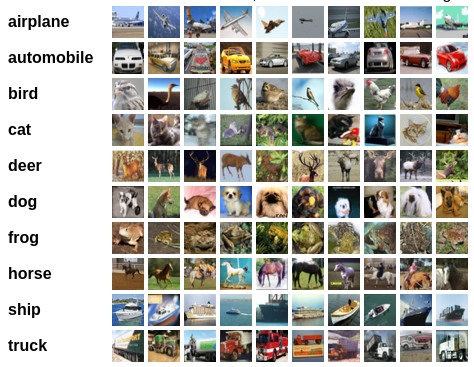
\includegraphics[width=0.7 \textwidth]{cifar-10.png}
		\caption{Przykładowe zdjęcia ze zbioru danych CIFAR-10. Każdy wiersz zdjęć zawiera zdjęcia z jednej klasy.}
		\label{cifar-example}
	\end{figure}

	\section{Liniowe klasyfikatory}
	\label{klas-lin}
	Jako pierwsze algorytmy uczenia maszynowego do rozpoznawania obrazów poznałem klasyfikatory liniowe. Skupiłem się na dwóch algorytmach: Softmax oraz wieloklasowy SVM, które opisuję w kolejnych sekcjach. Klasyfikatory liniowe opisuje funkcja liniowa:

	$$
		f(x_i, W, b) = Wx_i + b
	$$

	W powyższej funkcji $x_i$ to wartości pikseli $i$-tego obrazu umieszczone w wektorze o wymiarach [D x 1], gdzie D to wymiarowość obrazka. Macierz $W$ oraz wektor $b$ to parametry funkcji, często określane jako macierz wag oraz wektor bias. macierz $W$ ma wymiary [K x D], gdzie K to ilość klas wyjściowych klasyfikatora. Wektor $b$ ma wymiary [K x 1]. W przypadku zbioru danych CIFAR-10 wektor $x_i$ ma wymiary [3072 x 1], wynika to z wymiarów pojedynczego obrazu wynoszących [32 x 32 x 3], macierz $W$ ma wymiary [10 x 3072], a wektor $b$ ma wymiary [10 x 1]. Parametry $W$ oraz $b$ wykształacane są podczas procesu uczenia.

	\textbf{Klasyfikator liniowy jako podział wielowymiarowej przestrzeni.} Wektory odpowiadające obrazom interpretować można jako punkty w wielowymiarowej przestrzeni(np. w przypadku zbioru CIFAR-10 jako punkt w 3072-wymiarowej przestrzeni). Zgodnie z definicją funkcji klasyfikującej do klas, wynik dla każdej klasy to ważona suma pikseli obrazu. Jeśli spróbowaliśmy przedstawić wszystkie wymiary zbioru danych w dwóch wymiarach wizualizacji tego, jak działa klasyfikator może wyglądać, tak jak na rysunku \ref{linear-clas}.

	\begin{figure}[h]
		\centering
		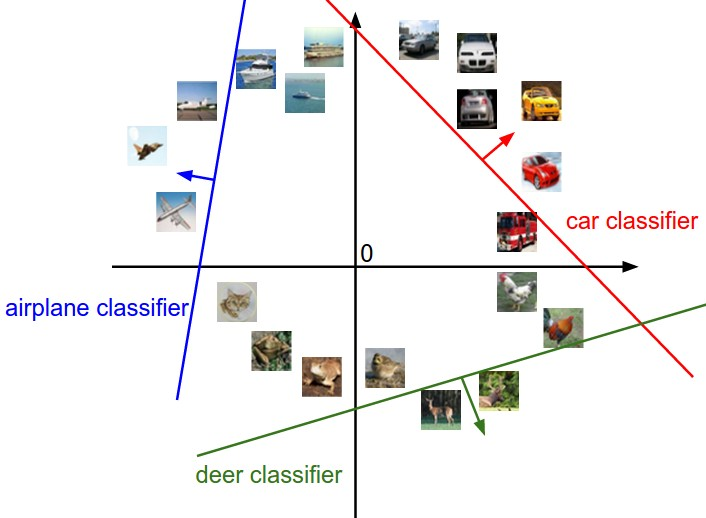
\includegraphics[width=0.9 \textwidth]{lin-clas.jpeg}
		\caption{Wizualizacja wielowymiarowej przestrzeni oraz granic klasyfikacji na dwóch wymiarach.}
		\label{linear-clas}
	\end{figure}

	\textbf{Klasyfikator liniowy jako dopasowanie do szablonu.} Inną interpretacją macierzy wag $W$ jest uznanie, że każdy rząd macierz $W$ opisuje szablon(prototyp) dla każdej z klas. W tym przypadku wynik dla każdej z klas to porównanie obrazu wejściowego z szablonem i sprawdzenie, dla której klasy występuje największe podobieństwo. Szablony(prototypy) tworzone są podczas procesu uczenia. 

	\begin{figure}[h]
		\centering
		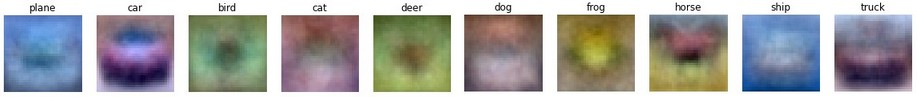
\includegraphics[width=1 \textwidth]{templates.jpg}
		\caption{Wizualizacja szablonów dla zbioru danych CIFAR-10.}
		\label{templates}
	\end{figure}

	Analizując powyższe prototypy można zauważyć, że dla klasy \texttt{horse} koń posiada dwie głowy, co może oznaczać, że w zbiorze danych znajduje się tyle samo zdjęć koni zwróconych w lewo jak w prawo. Klasyfikator liniowy przyporządkowuje tylko jeden szablon, więc nie sklasyfikuje prawdopodobnie samochodu innego koloru niż czerwony, patrząc na szablon klasy \texttt{car}.

	\textbf{Funkcja kosztu.} Jakość klasyfikacji podczas uczenia oceniać będziemy za pomocą funkcji kosztu. Docelowo będzie ona zmniejszać wraz z postępem uczenia klasyfikatora.

	\subsection{Wieloklasowy klasyfikator SVM}
	Przykładem klasyfikatora liniowego jest wieloklasowy klasyfikator SVM, nazywany również maszyną wektorów nośnych. Klasyfikator SVM stara się przyporządkować poprawnej klasie przyporządkować wynik wyższy o pewnien margines $\Delta$. Podstawową formę funkcji koszu wieloklasowego SVM można zapisać:
	
	$$
		L_i = \sum_{j\neq y_i} max(0, s_j - s_{y_i} + \Delta) 
	$$

	Wzór można rozwinąć o szczegółowe określenie obliczania wyniku $s$, w przypadku liniowej funkcji wyniku wygląda to:

	$$
		L_i = \sum_{j\neq y_i} max(0, w^T_jx_i - w^T_{y_i}x_i + \Delta) 
	$$

	\textbf{Regularyzacja.} W celu nadmiernego dopasowania się macierzy wag $W$ stosuje się parametr regularyzacji. Najczęściej używa się regularyzacji normą $L2$, jej zadaniem jest ograniczenie dużych wag. Funkcja kosztu SVM wraz z paramterem regularyzacji wygląda:

	$$
		L = \frac{1}{N} \sum_{i} L_i + \lambda R(W)
	$$

	W pełnej formie funkcję kosztu można zapisać:

	$$
		L = \frac{1}{N} \sum_{i} \sum_{j\neq y_i}[max(0, w^T_jx_i - w^T_{y_i}x_i + \Delta) ] + \lambda R(W) + \lambda\sum_{k}\sum_{l} W^2_{k,l}
	$$

	Hiperparametr $\lambda$ dobierany jest podczas walidacji krzyżowej. 

	\subsection{Klasyfikator Softmax}
	Klasyfikator Softmax jest generalizacją binarnej regresji logistycznej pozwalającą na klasyfikację wielu klas. Funkcję kosztu dla tego klasyfikatora można zapisać jako:

	$$
		L_i = -\log\left(\frac{e^{f_{y_i}}}{\sum_{j} e^{f_{y_i}}}\right)
	$$

	\textbf{Interpetacja w teorii informacjii.} Entropia krzyżowa między \textit{prawdziwą} dystrybucją $p$ i estymowaną dystrybucją $q$ może zostać zdefiniowana:

	$$
		H(p,q) = -\sum_{x}p(x)\log q(x)
	$$

	Klasyfikator Softmax minimalizuje entropię krzyżową między estymowanym prawdopodobieństwem przynależności do klas i \textit{prawdziwą} dystrybucją, która interpretowana jest jako dystrybucja, gdzie prawdopodobieństwo przynależności do poprawnej klasy wynosi 1.

	\textbf{Interpretacja w teorii prawdopodobieństwa.} Klasyfikator Softmax może być interpretowany jako prawdopodobieństwo przyporządkowania do klasy $y_i$, pod warunkiem obrazu $x_i$, parametryzowane przez macierz $W$. Zapisać można to:

	$$
		P(y_i|x_i;W)=\frac{e^{f_{y_i}}}{\sum_{j} e^{f_{y_i}}}
	$$

	\section{Sieci neuronowe}
	Sieci neuronowe to algorytmy zainspirowane budową mózgu oraz naturalnymi sieciami neuronowymi. Starają się one symulować model mózgu poprzez odpowiedni model matematyczny. Na rysunkach poniżej widać zestawienie modelu neuronu z mózgu biologicznego z neuronem ze sztucznej sieci neuronowej.

	\begin{figure}[h!]
        \centering
        \begin{subfigure}{.5\textwidth}
          \centering
          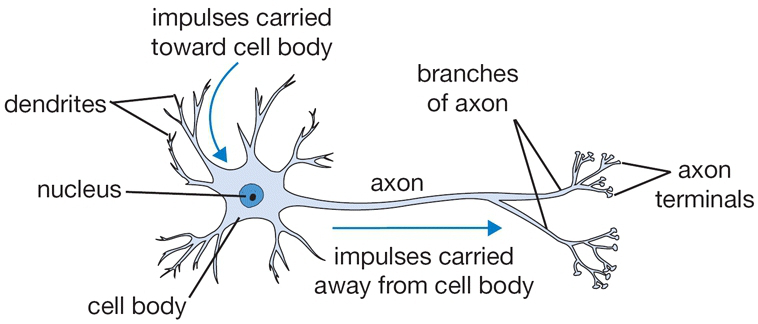
\includegraphics[width=.95\linewidth]{brain.png}
          \caption{Neuron z mózgu naturalnego.}
          \label{fig:sub1}
        \end{subfigure}%
        \begin{subfigure}{.5\textwidth}
          \centering
          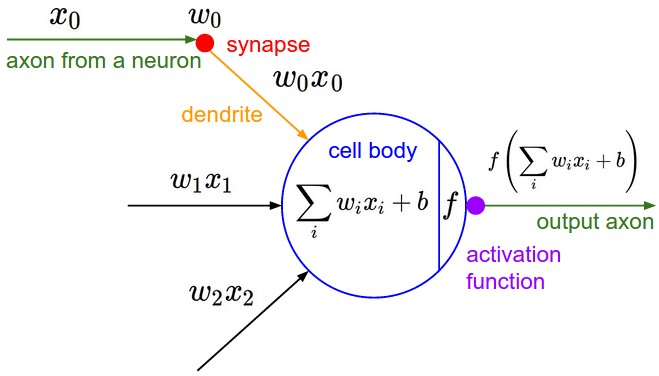
\includegraphics[width=0.95\linewidth]{neuron_model.jpeg}
          \caption{Neuron ze sztucznej sieci neuronowej.}
          \label{fig:sub2}
        \end{subfigure}
        % \caption{Wykres przedstawiający dane opisane przez dwa pierwsze składniki dla obu algorytmów.}
        \label{fig:vs}
	\end{figure}
	
	\textbf{Wprowadzenie.} Klasyfikator liniowy opisany w sekcji \ref{klas-lin} oblicza wynik dla klasy za pomocą formuły $s = Wx$. Sieć neuronowa obliczy wynik jako $s = W_2 \max(0, W_1 x)$. W tym przypadku macierz $W_1$ może być macierzą o wymiarach [3072 x 100] przekształcającą obraz w 100-wymiarowy wektor. Funkcja $\max(0,-)$ jest nieliniowością odnoszącą się do każdego elementu. Istnieje wiele nieliniowości, zostały one opisane poniżej. Macierz $W_2$ jest wymiaru [10 x 100], posiada ona wyniki dla każdej z 10 klas wyjściowych. Parametry $W_1$ oraz $W_2$ uczone są poprzez algorytm Stochastic Gradient Descent, a gradienty znajdowane są za pomocą reguły łańcuchowej, korzystając z propagacji wstecznej. 
	
	\textbf{Funkcje aktywacji.} W praktyce stosowane jest kilka rodzajów funkcji aktywacji, m. in. funkcja Sigmoid, Tanh, ReLU, Leaky ReLU oraz Maxout. Najczęściej stosowana jest funkcja ReLU, ponieważ zapewnia ona lepszą zbieżność gradientu od funkcji Sigmoid oraz Tanh. Jest ona również mniej złożona obliczeniowo.

	\textbf{Architektura sieci neuronowej.} Sieci neuronowe mogą być interpretowane jako zbiór połączonych neuronów w skierowanym grafie acyklicznym. Wyjścia części neuronów stają się wejściami innych. Modele sieci neuronowych są najczęściej zorganizowane jako warstwy neuronów. Najczęściej używa się w pełni połączonych warstw, w których wszystkie neurony są połączone parami pomiędzy obiema warstwami. Przykłady takich sieci zaprezentowane są poniżej.

	\begin{figure}[h!]
        \centering
        \begin{subfigure}{.5\textwidth}
          \centering
          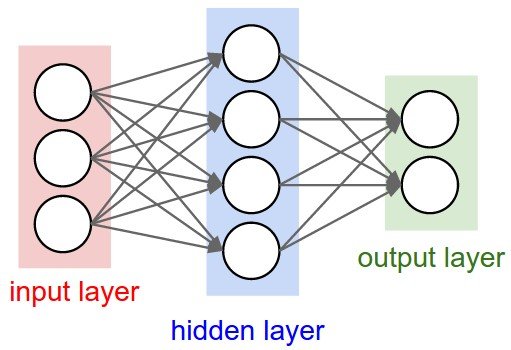
\includegraphics[width=.95\linewidth]{neural_net.jpeg}
          \caption{Sieć neuronowa z jedną warstwą ukrytą.}
          \label{fig:sub1}
        \end{subfigure}%
        \begin{subfigure}{.5\textwidth}
          \centering
          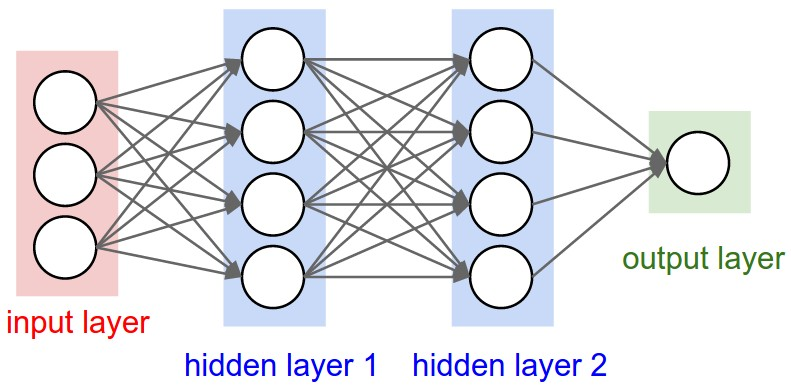
\includegraphics[width=0.95\linewidth]{neural_net2.jpeg}
          \caption{Sieć neuronowa z dwiema warstwami ukrytymi.}
          \label{fig:sub2}
        \end{subfigure}
        % \caption{Wykres przedstawiający dane opisane przez dwa pierwsze składniki dla obu algorytmów.}
        \label{fig:vs}
	\end{figure}

	\chapter{Splotowe sieci neuronowe}
	Za punkt odnesienia jakości algorytmów rozpoznawania obrazów bardzo często uznawało się konkurs Large Scale Visual Recognition Challenge (ILSVRC). Był to konkurs polegający na porównaniu algorytmów rozpoznawania obrazów oraz lokalizacji obiektów działających na zbiorze danych ImageNet \cite{imagenet_cvpr09}. Algorytmy biorące udział w historycznych edycjach poprawiały stopniowo błąd klasyfikacji, jednak nie były w stanie poprawić wyniku w znaczący sposób. W 2012 roku wynik poprawił się z 26\% na 16.4\% błędu. Stało się to za sprawą nowej architektury sieci neuronowej nazwaną splotową siecią neuronową (convolutional neural network).

	\begin{figure}[h!]
		\centering
		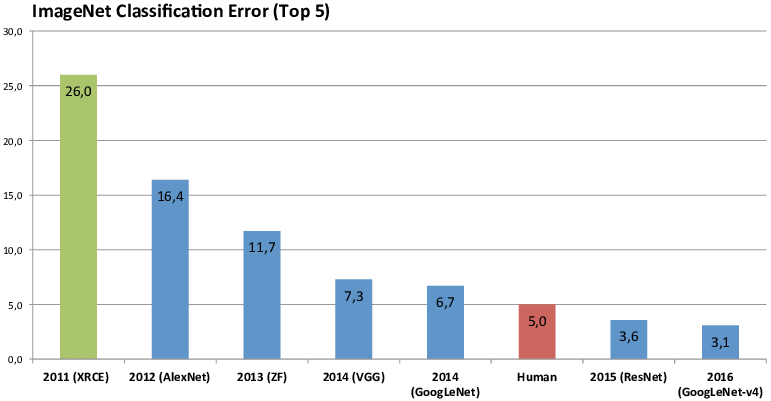
\includegraphics[width=1 \textwidth]{imnet.png}
		\caption{Wyniki konkursu ILSVRC w latach 2011 - 2016.}
		\label{imnet}
	\end{figure}

	Sieć nazywała się AlexNet i została opisana w artykule \cite{NIPS2012_4824}. Sieć splotowa jest bardzo zbliżona do zwykłej sieci neuronowej opisanej wcześniej. Różnicą jest to, że splotowa zakłada, że obiektem wejściowym będzie obraz, co pozwala na dostosowanie architektury. Zmniejsza również znacznie liczbę parametrów sieci.

	% \begin{figure}[h!]
	% 	\centering
	% 	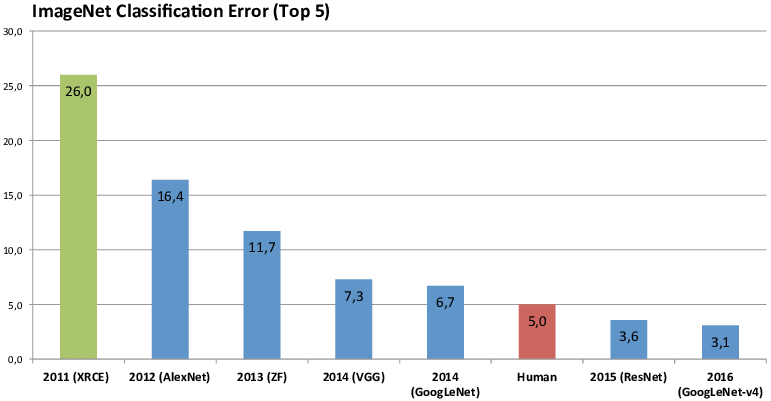
\includegraphics[width=1 \textwidth]{imnet.png}
	% 	\caption{Wyniki konkursu ILSVRC w latach 2011 - 2016.}
	% 	\label{imnet}
	% \end{figure}

	\textbf{Porównianie regularnych sieci neuronowych oraz sieci splotowych.}

	Regularne sieci neuronowe nie skalują się dobrze do obrazów. Dla przykładu zbiór CIFAR-10 zawiera obrazy wielkości 32x32x3, więc jedna w pełni połączona warstwa sieci neuronowej posiada 32*32*3 = 3072 parametrów. Nie jest to liczba, która wyklucza użycie tej warstwy ze względów złożoności, jednak problem nasila się w przypadku większych obrazów. Obraz o wielkości 200x200x3 będzie posiadał 120000 paramterów. Dodatkowo, chcielibyśmy użyć kilku takich warstw, co powoduje znaczne zwiększenie liczby parametrów. Tak duża liczba paramterów może powodować przeuczenie.

	Sieci splotowe pozwalają na trójwymiarowość neuronów. Warstwy sieci splotowe posiadają neurony zorganizowane w trzech wymiarach: szerokość, wysokość oraz głębokość. Struktura warstwy widoczna jest na rysunku \ref{convlay}.
	
	\begin{figure}[h]
		\centering
		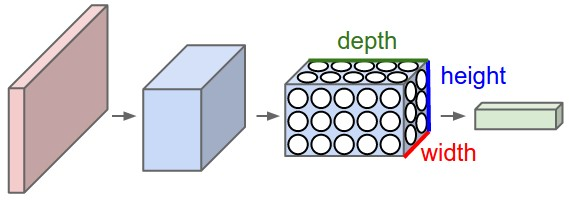
\includegraphics[width=0.7\textwidth]{cnn.jpeg}
		\caption{Struktura neuronów w sieci splotowej.}
		\label{convlay}
	\end{figure}

	\section{Warstwy w sieci splotowej}
	Sieć splotowa tak jak sieć neuronowa składa się z warstw. W praktyce używa się trzech typów warstw: warstw splotowe (Convolutional Layer), warstw łączących (Pooling Layer) oraz warstw w pełni połączonych (Fully-Connected Layer). 

	\textbf{Przykładowa architektura.} Prosta sieć splotowa dla zbioru danych CIFAR-10 może składać się z następujących warstw:

	\begin{itemize}
		\item INPUT [32x32x3] przechowuje wartości wejściowe pikseli obrazu, mającego w tym przypadku wysokość 32, szerokość 32 oraz 3 kolory R,G,B.
		\item CONV wyznaczy wartości dla neuronów połączonych regionami w warstwie wejściowej, dla każdego obliczając produkt mnożenia macierzy parametrów oraz regionu wejściowego. Może zwracać wynik w postaci [32x32x12], jeżeli zostanie użyte 12 filtrów.
		\item RELU wyznaczy wartości funkcji aktywacji, np. $\max(0,x)$. Wyniki pozostaną w postaci [32x32x12].
		\item POOL wykona operację próbkowania, zmniejszając wymiary wysokości i szerokości. Wyniki będą w postaci [16x16x12].
		\item FC wyznaczy wyniki dla klas, zwracając wyniki wielkości [1x1x10]
	\end{itemize}

	\textbf{Warstwa splotowa.} Warstwa CONV zawiera zbiór filtrów, których parametry zmieniają się podczas uczenia. Filtr posiada małe wymiary wysokości oraz szerokości, ale przetwarza całą głębokość obrazu. Dla przykładu typowy filtr pierwszej warstwy może mieć wymiary [5x5x3]. Filtr ten będzie \textit{przesuwany} po obrazie, zwracają produkt mnożenia macierzy regionu wejściowego oraz paramterów filtru. Wynik działania będzie dwuwymiarową mapą odpowiedzi filtru na każdej pozycji w przestrzeni. Sieć w miarę uczenia wykształci filtry, które aktywują się na takie cechy jak brzegi na obrazie. 

	Podczas analizy danych wielowymiarowych, takich jak obrazy, nie jest zalecane, aby każdy neuron był połączony ze wszystkimi neuronami z warstwy poprzedniej. Zamiast tego stosuje się połączenie każdego z neuronów z małym regionem danych wejściowych. 

	\begin{figure}[h]
		\centering
		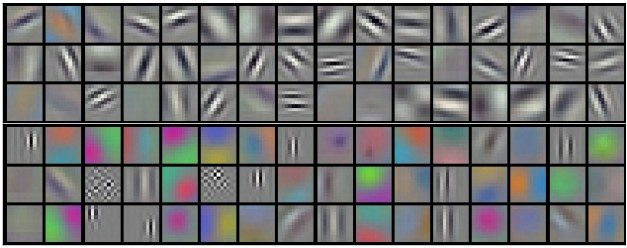
\includegraphics[width=1\textwidth]{filters.jpeg}
		\caption{Przykładowe filtry pierwszej warstwy w sieci AlexNet. Każdy z 96 filtrów ma wymiary [11x11x3]. Podział na filtry szrości oraz koloru wynika z architektury sieci ALexNet i podziału potoków przetwarzania.}
		\label{convlay}
	\end{figure}

	\textbf{Warstwa próbkująca.} W praktyce umieszcza się warstwy próbkujące między warstwami splotowymi. Pozwalają one na zmniejszanie wymiarów szerokości i wysokości w celu ograniczenia liczby parametrów oraz obliczeń w sieci. Zmniejszają również podatność na przeuczenie. Najczęściej stosowana jest warstwa z filtrem o wymiarach [2x2] aplikowana z krokiem 2 z użyciem operacji pobierania największego elementu. Pozwala to ograniczyć liczbę parametrów o 75\%. Głębokość pozostaje niezmieniona.

	\subsection{Sieć VGGNet}
	Jedną z najczęsciej używanych sieci jest sieć VGGNet \cite{SimonyanZ14a} biorąca udział w ILSVRC 2014. Zawiera ona 16 warstw CONV/FC. Stosowane są w niej jedynie filtry 3x3 oraz próbkowanie 2x2. Poniżej zaprezentowana jest w pełni architektura sieci VGGNet. Sieć posiada 138 milionów parametrów oraz zajmuje 93 MB pamięci (jedynie dla propagacji w przód) dla jednego obrazu o wymiarach [224x224x3].

	\begin{figure}[h]
		\centering
		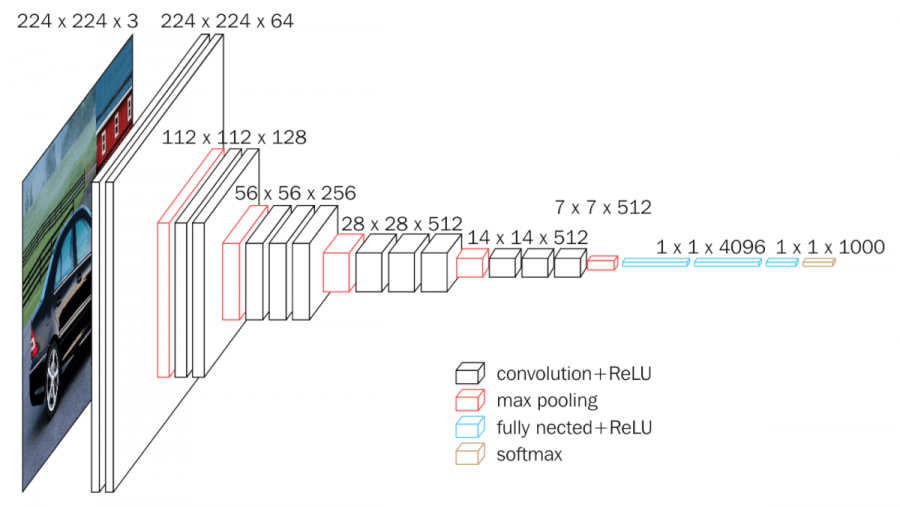
\includegraphics[width=1\textwidth]{vgg16.png}
		\caption{Architektura sieci VGG.}
		\label{vgg}
	\end{figure}

	\section{Transfer Learning}
	W praktyce mała grupa ludzi trenuje sieci splotowe od zera, głównie ze względu na nieposiadanie odpowiednio dużego zbioru danych. Częste jest użycie wcześniej wyuczonej sieci na bardzo dużym zbiorze danych (np. zbiór ImageNet), a następnie użycie sieci jako punkt wyjścia do własnego dostrojenia lub jako narzędzie do wyodrębniania cech. Stosuje się trzy sposoby Transfer Learning:

	\begin{itemize}
		\item \textbf{Sieć splotowa jako narzędzie do wyodrębniania cech.} Po usunięciu ostatniej w pełni połączonej warstwy sieć splotowa może służyć jako narzędzie do wyodrębniania cech do nowego zbioru danych. Cechy te nazywane są kodami CNN.
		\item \textbf{Dostrajanie sieci splotowej.} Istnieje możliwość dostrojenia wytrenowanej sieci splotowej do własnego zbioru danych poprzez propagacje wsteczną. Możliwe jest dostrojenie wszystkich warstw sieci, jednak najczęściej początkowe warstwy pozostawia się w stałej postaci i dostraja jedynie warstwy dalsze. Wynika to z obserwacji mówiących, że początkowe warstwy sieci zawierają bardziej ogólne cechy (np. brzegi oraz skupienia kolorów) i są przydatne w większości problemów. Późniejsze warstwy stają się coraz bardziej specyficzne dla klas w danym zbiorze.
		\item \textbf{Wyuczone modele.} Wyuczenie nowoczesnej sieci splotowej wymaga od 2 do 3 tygodnie uczenia na wielu kartach graficznych na zbiorze ImageNet. W związku z tym wiele ludzi udostępnia wytrenowane przez nich sieci splotowe, z których mogą skorzystać inni. Przykładem może być biblioteka Caffe, która udostępnia Model Zoo.
	\end{itemize}


	\chapter{Wykrywanie współwystępowania} 

	Wykrywanie współwystępowania obiektów (z ang. co-saliency detection) to względnie nowy problem dziedziny przetwarzania obrazów cyfrowych. Jako nowy dział wykrywania istotności na obrazach (saliency detection), zajmuje się poszukiwaniem częstych i istotnych regionów w grupie kilku obrazów. Obecne algorytmy wykrywania współwystępowania obiektów składają się najczęściej z trzech części: wyodrębnienia odpowiednich cech w celu reprezentacji obiektów na obrazie, analizy czynników  charakteryzujących współwystępowanie oraz stworzenia efektywnego obliczeniowo systemu do wyznaczania współwystępowania obiektów. 

	\section{Opis problemu}
	Wykrywanie istotności (saliency detection) stara się zrozumieć sposób w jaki ludzie postrzegają dane wizualane, takie jak obrazy, poprzez wykrywanie obszarów na które ludzie zwracają najwięcej uwagi. Zagadnienie wykrywania współwystępowania obiektów (co-saliency detection) stara się wykryć występowanie powtarzalnych oraz istotnych (w sensie postrzegania przez człowieka) regionów w grupie powiązanych ze sobą obrazów. Wykrywanie współwystępowania znajduje swoje zastosowanie jako element przygotowania danych w wielu aplikacjach, takich jak wspólna segmentacja kilku obrazów lub filmu, lokalizacja obiektów, analiza nagrań z kamer bezpieczeństwa oraz wyszukiwanie za pomocą obrazów. 

	Algorytmy wykrywania współwystępowania obiektów można podzielić za względu na reprezentacje cech. Duża część algorytmów, np. \cite{ChangLL11}, wykorzystuje cechy niskiego poziomu, takie jak histogramy koloru, filtry Gabor oraz deskryptory SIFT. Metody te zakładają, że współwystępujące obiekty są ze sobą spójne na poziomie cech niskiego poziomu. Kolejna grupa metod, np. \cite{midfeatex}, używa dodatkowo cech średniego poziomu w celu wykrywania współwystępowania. Te metody korzystają zazwyczaj z wyników algorytmów wykorzystujących cechy niskiego poziomu i traktują je jako cechy średniego poziomu, zakładając spójność tych cech w grupie obrazów. Obecnie najwięcej algorytmów, np. \cite{highfeatex}, stosuje cechy wysokiego poziomu, zakładając ich spójność w grupie zdjęć. W ramach algorytmów wykrywania współwystępowania za cechy niskiego poziomu uważa się zazwyczaj te cechy, które odnoszą się do wartości pojedynczych pikseli. Cechy średniego poziomu odnoszą się do map generowanych przez istniejące metody wykrywania współwystępowania. Cechy wysokiego poziomu odnoszą się do cech zawierające znaczące informacje o danych. Dotyczy to najczęściej cech otrzymywanych z warstw głębokich sieci splotowych. 
	
	% Znanym problemem w dziedzinie wykrywania współwystępowania obiektów jest reprezentacja cech pikseli oraz obszarów. Używane były tradycyjne metody, takie jak histogram koloru, filtry Gabor oraz deskryptory SIFT. Wyniki uzyskane za pomocą tych metod są jednak w większości niezadawalające (feature discrimination). Niedawno metody uczenia głębokiego powoliły na uzyskanie znacznie lepszej skuteczności, ponieważ pozwalają na uzyskanie lepiej opisujących cech. Kolejnym zadaniem dzedziny jest wykrywanie powtarzających się regionów o dużej istotności na wielu obrazach. Zrealizowane jest to poprzez użycie odpowiedniej strategii asocjacyjnej. Metody wykorzystujące uczenie nienadzorowane używają klasteryzacji oraz modeli graficznych(?). Modele uczenia nadzorowanego wytrenowane do wykrywania istotności (saliency) również mogą być wykorzystywana do wykrywania współwystępowania. Wadą tego podejścia jest igonorwanie wzoru obszarów istotnych powtarzającego się w grupie obrazów. Niesie to ze sobą zanik różnic między zadaniem wykrywania istotności (saliency detection) oraz wykrywaniem współwystępowania (co-saliency detection). W celu rozwiązania tego problemu zostały użyte rozwiązania modelujące powtarzanie się wzoru między obrazami. Wykorzystane zostały metody takie jak metric learning oraz collaborative learning.

	\begin{figure}[h]
		\centering
		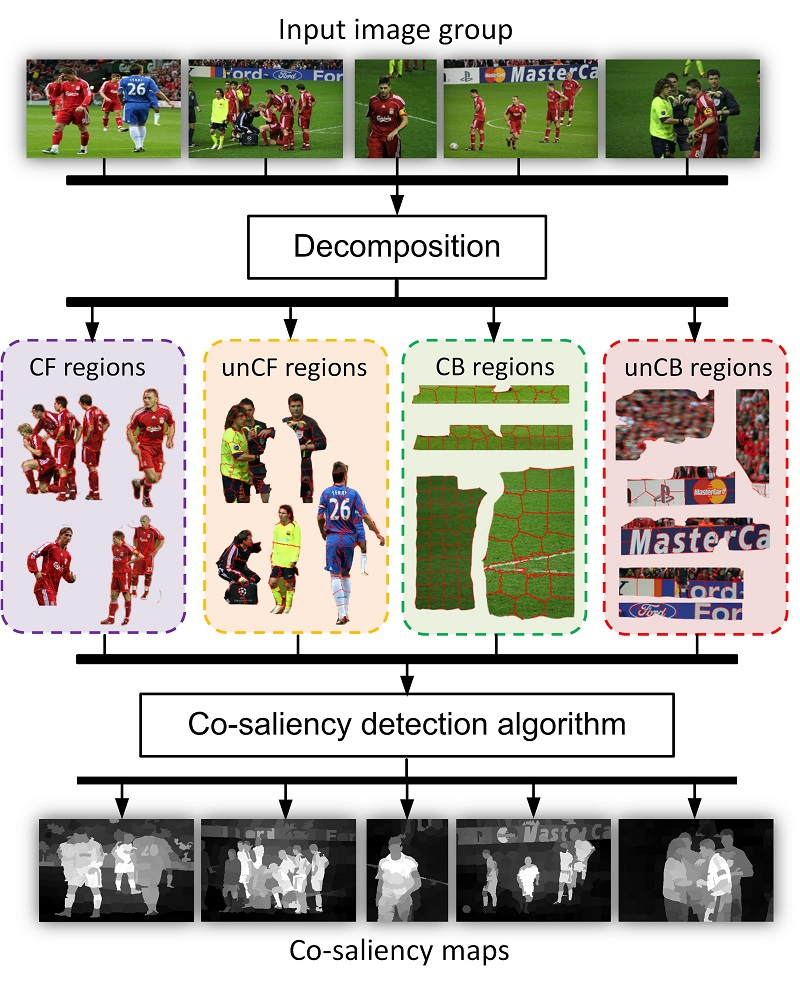
\includegraphics[width=0.6\textwidth]{cosaliency.png}
		\caption{Przykład podziału grupy obrazów na obszary powtarzające się. Zadaniem algorytmu wykrywania współwystępowania jest stworzenie mapy współwystępowania pokazującej wspólne obszary istotności.}
		\label{co}
	\end{figure}

	\section{Przegląd metodyki}
	W zakresie wykrywania współwystępowania obiektów wyróżnia się trzy podejścia do tworzenia algorytmów: podejście oddolne, podejście łączące oraz podejście oparte na uczeniu.

	\begin{figure}[h]
		\centering
		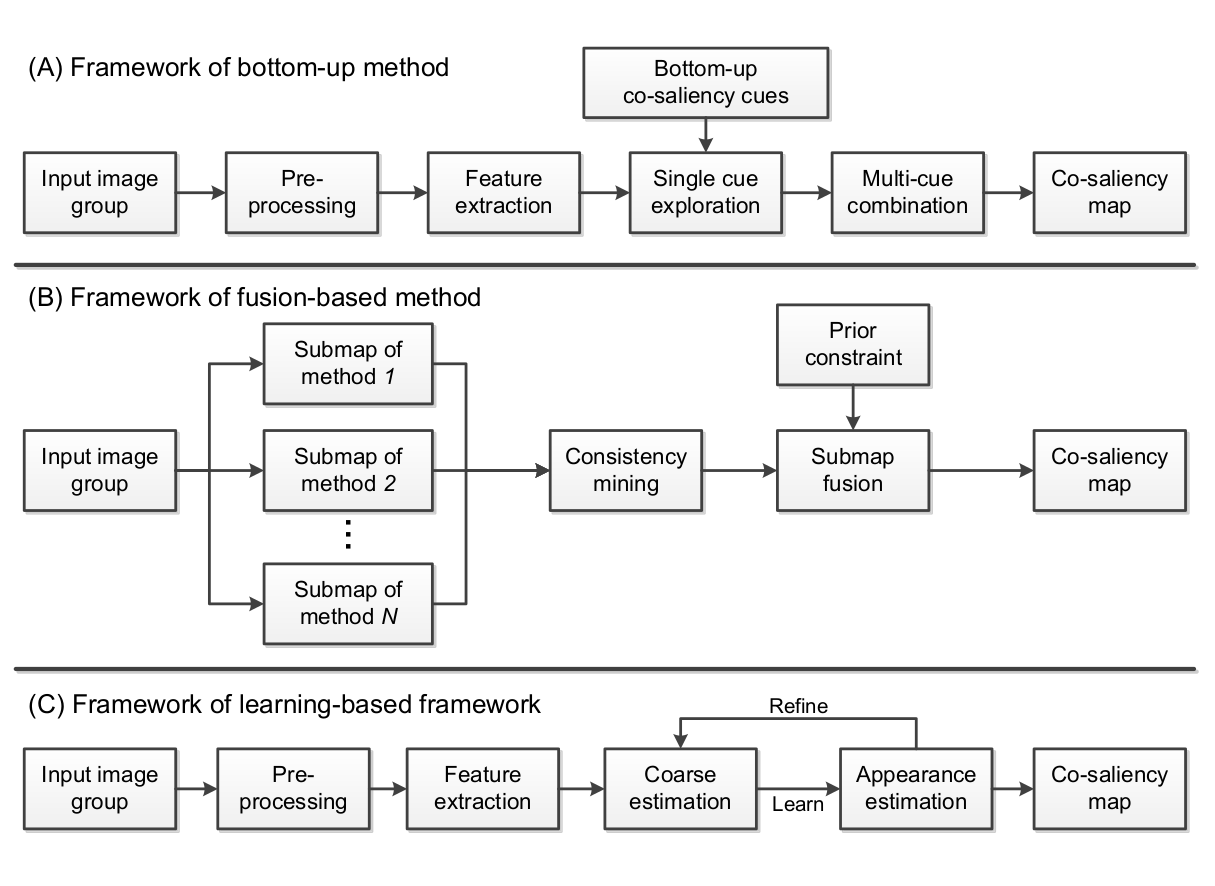
\includegraphics[width=1\textwidth]{cosal_met.png}
		\caption{Podział algorymtów wykrywania współwystępowania.}
		\label{pod}
	\end{figure}

	\subsection{Podejście oddolne}
	Pierwsza z omawianych metod skupia się na określeniu wyniku dla każdego pikseli w grupie obrazów korzystając z wcześniej określonych metryk istotności. Na rysunku \ref{pod} (A) przedstawiony jest schemat blokowy algorytmu wykorzystującego podejście oddolne. Składa on się takich kroków, jak: przygotowanie danych, wyodrębnienie cech, analiza pojedynczych metryk istotności oraz analiza kombinacji wielu metryk. Krok przygotowania danych obejmuje podział obrazu wejściowego na pojedyncze obiekty (np. piksele, klastry pikseli lub segmenty superpikseli). Następnie wyodrębniane są cechy każdego obiektu w celu ustalenia jego właściowści w oparciu o wcześniej stworzone metryki istotności. Ostatnim krokiem jest połączenie map istotności dla całej grupy obrazów za pomocą metryk współwystępowania, których stworzenie jest głównym problemem podzas tworzenia tego rodzaju metod. W ogólności metryki współwystępowania można opisać jako:

	$$
		\text{Co-saliency} = \text{Saliency} \times \text{Repeatedness}
	$$

	% Co w tłumaczeniu na język polski można zapisać:

	% $$
	% 	Współwystępowanie = Istotność \times Powtarzalność
	% $$

	Do analizy metryk używane są różne techniki, m. in. matrix factorization oraz pattern mining. 

	Jedną z najczęściej stosowanych metod oddolnych, jest taka, która wykorzystuje mechanizm klasteryzacji oparty o trzy metryki istotności. Dla każdego klastra $t$ jego współwystępowanie określone jest jako:

	$$
		\text{Co-saliency}^t = Cue^t_{Con} \times Cue^t_{Spa} \times Cue^t_{Corr}
	$$

	gdzie

	$$
		Cue^t_{Con} = \sum_{\tau \neq t} \frac{n^\tau}{N}\left(\|\mathbf{u}^\tau - \mathbf{u}^t\|_2\right)
	$$
	$$
		Cue^t_{Spa} = \frac{1}{n^t}\sum_{p \in C_t} \mathcal{N}\left(\|\mathbf{z}_p - \mathbf{o}_p\|_2|0,\sigma^2\right)
	$$
	$$
		Cue^t_{Corr} = 1/\left(\text{Var}\left(\mathbf{q}^t\right)+1\right)
	$$

	gdzie $Cue^t_{Con}$, $Cue^t_{Spa}$ i $Cue^t_{Corr}$ oznaczają odpowiednio metryki kontrastu, przestrzeni oraz zgodności. $\mathbf{u}^t$, $n^t$ oraz $\mathbf{q}^t$ oznaczają odpowiedznio centrum klastra, liczbę pikseli oraz dystrybujcę klastra $C_t$. Estymator jądrowy gęstości o jądrze normalnym $\mathcal{N}(\cdot)$ służy do wyznaczenia metryki euklidesowej pomiędzy $\mathbf{z}_p$ (współrzędnymi piksela p) oraz współrzędnymi centrum odpowiedniego obrazu $\mathbf{o}_p$. $\text{Var}\left(\mathbf{q}^t\right)$ oznacza wariancję histogramu $\mathbf{q}^t$. Algorytm jest dokładniej opisany w \cite{bott}.

	Metody wykorzystujące podejście oddolne są najczęściej używane w zadaniu wykrywania współwystępowania. Problemem tych metod jest jednak potrzeba ręcznego stworzenia odpowiednich metryk istotności. Metryki te są najczęściej zbytnio dostosowane do konkretnego zadania i słabo radzą sobie z generalizacją.

	\subsection{Podejście łączące}
	Metody stosujące to podejście starają się wydobyć informacje o współwystępowaniu z wyników istniejących już algorytmów wykrywania istotności lub współwystępowania. Łączą te wyniki oraz zdobytą wiedzę, aby generować wynikowe mapy współwystępowania. Na rysunku \ref{pod} (B) przedstawiony jest schemat blokowy algorytmu wykorzystującego podejście łączące. Pierwszym krokiem jest wygenerowanie map poprzez użycie istniejących algorytmów na danym zbiorze obrazów. Następnie poszukuje się powtarzalności pośród wygenerowanych map. W celu wyznaczenia wag połączenia map stosowane są ograniczenia ułatwiające ten proces. W ostatnim kroku wyznaczone wcześniej mapy łączone są w celu wygenerowania ostatecznych map współwystępowania:

	$$
	\text{Co-saliency} = \sum_i \text{Weight}_i \cdot \text{Submap}_i
	$$

	Typowym podejściem wykorzystującym to podejście jest \cite{midfeatex}. Mając macierz cech $\mathbf{H} = [\mathbf{H}^1, \mathbf{H}^2, \dots, \mathbf{H}^K]^T \in R^{M x D}$, $K$, $M$ oraz $D$ oznaczają odpowiednio liczbę obrazów, liczbę wyznaczonych map dla każdego obrazu oraz wymiar danej cechy. Powtarzalność pomiędzy tymi mapami może być wyznaczona jako:

	$$
	\arg\min_{\mathbf{L}, \mathbf{E}} \left(\|\mathbf{L}\|_* + \lambda\|\mathbf{E}\|_1\right)
	$$

	$$
	\mathbf{H} = \mathbf{L} + \mathbf{E}
	$$

	gdzie $\|\cdot\|_*$ oznacza normę macierzy, a $\|\cdot\|_1$ jej normę $l_1$. Macierz $\mathbf{E}$ jest macierzą błędów między macierzą $\mathbf{H}$ oraz macierzą rang $\mathbf{L}$, gdzie $\mathbf{E}^k=[\mathbf{e}^k_1, \mathbf{e}^k_2, \dots, \mathbf{e}^k)M]^T \in R^{M x D}$ jest macierzą błędu $k$-tego obrazu. Zatem waga $w^k_j$ dla $j$-tej mapy $k$-tego obrazu może zostać wyznaczona jako:

	$$
	w^k_j = \frac{\exp(\zeta^k_j)}{\sum^M_{j=1}\exp(\zeta^k_j)}
	$$

	$$
	\exp(\zeta^k_j) = -\|e^k_j\|_2
	$$
	
	Metody wykorzystujące podejście łączące zazwyczaj osiągają wyniki pozwalające sądzić, że są w stanie rozwinąć się korzystając z istniejących algorytmów wykrywania współwystępowania. Kolejnym plusem tej grupy algorytmów jest fakt, że istnieje możliwość dodania ich jako kolejna warstwa w procesie przetwarzania, w którym zaimplementowane są już algorytmy wykrywania współwystępowania. Ich wadą jest jednak to, że opierają swoje działania o istniejące algorytmy wykorzystujące podejście oddolne, powielając wady tej grupy algorymtów.

	\subsection{Podejście oparte o uczenie}
	Trzecią grupą algorymtów są metody oparte na uczeniu. Dążą one do wyuczenia się wzorów współwystępowania z danej grupy obrazów. Wspomniane wcześniej dwie grupy metod również mogą wykorzystywać uczenie maszynowe podczas konkretnych kroków, ale nie używają tej techniki do wyznaczania mapy współwystępowania. Na rysunku \ref{pod} (C) przedstawiony jest schemat blokowy algorytmu opartego o uczenie. Cechą charakterystyczną tej metody jest wykorzystanie algorytmu uczenia nienadzorowanego do wyznaczenia początkowej mapy współwystępowania. Kolejnym krokiem jest iteracyjne uczenie się algorytmu w celu poprawy wyznaczonej mapy współwystępowania.

	Przykładem z algrytmu z tej grupy może być algorytm opisany w \cite{10.1109/TPAMI.2016.2567393}. Zakładamy, że mamy grupę zdjęć $K_+$ opisaną jako zbiór pozytywny oraz wyszukaną grupę zdjęć $K_-$ opisaną jako zbiór negatywny. Dla każdego obrazu wyznaczamy superpiksele wraz z reprezentacją cech $\mathbf{x}_i^{(k)}$, które traktowane są jako obiekty do klasyfikacji, gdzie $k \in [1, K]$, $K=K_+ + K_-$ oznacza index w zbiorze dla każdego obrazu, a $i \in [1, n_k]$ oznacza indeks superpiksela obiektu dla każdego $k$-zbioru. Funkcja kosztu jest zdefiniowana jako:

	$$
		\min_{\mathbf{w},b,\mathbf{y}^{(1)}, \dots, \mathbf{y}^{(K_+)},\mathbf{v}\in[0,1]^n} E(\mathbf{w},b,\mathbf{y}^{(1)}, \dots, \mathbf{y}^{(K_+)},\mathbf{v}) = 
	$$

	$$
	\frac{1}{2} \|\mathbf{w}\|^2_2 + \sum_{k=1}^K \sum_{i=1}^{n_k}v_i^{(k)} L(y_i^{(k)}, g(\mathbf{x}^{(k)}_i;\mathbf{w},b)) + f(\mathbf{v};\lambda, \gamma)
	$$

	$$
	\|\mathbf{y}^{(k)}+1\|_0 \geq 1, k=1,2,\dots,K_+
	$$

	gdzie $\mathbf{v} = [v_1^{(1)}, \dots, v_{n_1}^{(1)}, v_{1}^{(2)}, \dots, v_{n_2}^{(2)}, \dots, v_{n_k}^{(K)}] \in R^{n}$ oznacza znaczenie wag dla obiektów, $\mathbf{y} = [y_1^{(k)}, y_{2}^{(k)}, \dots, y_{n_k}^{(k)}] \in R^{n_k}$ oznacza etykiety dla obiektu $k$-tego zbioru, $L(y_i^{(k)}, g(\mathbf{x}^{(k)}_i;\mathbf{w},b))$ oznacza funkcję kosztu $\mathbf{x}_i^{(k)}$ dla klasyfikatora SVM $g(\mathbf{x}^{(k)}_i;\mathbf{w},b)$ z~wektorem wag $\mathbf{w}$ oraz parametrem bias b. Ograniczenie powoduje, że będzie istniał przynajmniej jeden pozytywny obiekt dla każdego pozytywnego zbioru. $f(\mathbf{v};\lambda, \gamma)$ jest funkcją regularyzacji.

	W przypadku algorytmów wykrywania współwystępowania tego rodzaju wiedza obiektach współwystępujących poznawana jest przez algorytm w procesie uczenia, zamiast w rezultacie ręcznie zaprojektowanych metryk. Algorytmy uczenia maszynowego są w stanie znaleźć bardziej skomplikowane zależności w danych od człowieka, ponieważ metryki wymyślane przez człowieka są najczęściej nadmiernie dostosowane do konkretnego zadania i mają słabą zdolność generalizacji. Wadą algorytmów opartych o uczenie jest czas potrzebny w etapie treningu.



	\section{Ocena algorytmów}
	\subsection{Zbiory danych}
	Algorytmy wykrywania współwystępowania sprawdzane są najczęściej na czterech publicznych zbiorach danych: Image Pair \cite{ImagePair}, iCoseg \cite{iCoseg}, MSRC \cite{MSRC} oraz Cosal2015 \cite{cosal2015}. Przykładowe obrazy z każdego zbioru przedstawione są na rysunku \ref{ds}. Porównanie zrealizowane jest w tabeli \ref{table}.

	\begin{figure}[h]
		\centering
		\includegraphics[width=1\textwidth]{datasets.png}
		\caption{Przykładowe obrazy ze zbiorów danych służących do oceny algorytmów wykrywania współwystępowania.}
		\label{ds}
	\end{figure}

	Zbiór danych Image Pair zawiera 105 par obrazów (razem 210 obrazów) o rozdzielczości 128x100 pikseli. Posiada ręcznie określane wartości prawdy i jest pierwszym zbiorem danych dla zadania wykrywania współwystępowania. Każda z par obrazów zawiera podobne obiekty znajdujące się na różnym tle. W tym zbiorze danych tło jest mniej zróżnicowane niż w innych zbiorach. Obecnie zbiór ten nie jest często używany, ponieważ nie jest wystarczająco wymagający dla nowoczesnych algorytmów.
	
	\begin{figure}[h]
		\centering
		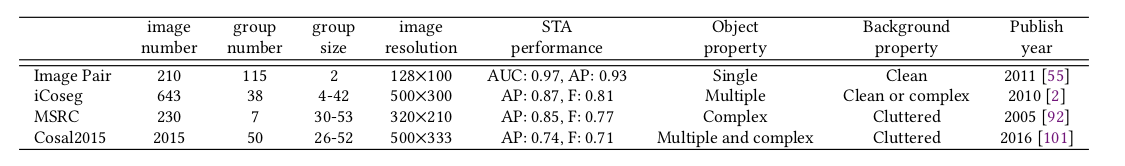
\includegraphics[width=1\textwidth]{ds_comp.png}
		\caption{Tabela przedstawiająca porównanie zbiorów danych.}
		\label{table}
	\end{figure}

	Zbiór iCoseg jest otwartym zbiorem danych. Posiada 38 grup obrazów (643 razem), jak również wartości prawdy dobrane ręcznie dla każdego piksela. W odróżnieniu od zbioru Image Pair grupy zawierają od 4 do 42 obrazów. Obrazy w tym zbiorze charakteryzują się najczęściej zróżnicowanym tłem oraz kilkoma obiektami na obrazie. Zbiór ten jest jednym z najczęsciej używanych podczas ewaluacji algorytmów wykrywania współwystępowania.

	Kolejnym często używanym zbiorem jest zbiór MSRC. Zawiera on 8 grup (razem 240 obrazów) wraz z prawdą ręcznie dobraną dla każdego piksela. Grupy obrazów to np. samoloty, rowery lub samochody. Istnieje również grupa zawierająca trawę, jednak nie jest ona zazwyczaj używana w zadaniu wykrywania współwystępowania obiektów, ponieważ ich nie zawiera.

	Najnowyszym zbiorem danych wsród tych używanych przy wykrywaniu współwystępowania obiektów jest zbiór Cosal2015. Posiada on 50 grup zdjęć (2015 razem) zebranych z konkursu ILSVRC2014 oraz filmów w serwisie YouTube. Tła obrazów w tym zbiorze są mocno zróżnicowane. Dodatkowo często na jednym obrazie znajduje się kilka obiektów istotnych, których część nie występuje na innych obrazach w grupie.

	\subsection{Miary oceny}
	Oceny algorytmów wykrywania współwystępowania można dokonać za pomocą sześciu przyjętych miar: krzywej PR (precyzja-czułość), średniej precyzji (AP), krzywej miary F, średniej miary F (mF), krzywej ROC oraz miary AUC. 

	Krzywa PR oraz miara AP wyznaczane są poprzez podział pikseli w mapie istostności na istotne oraz nieistotne. W rezultacie miara czułości zestawiona z miarą precyzji tworzy krzywą PR. Pole pod krzywą wyznacza miarę średniej prezyzji (AP). Krzywa ROC jest wyznaczana w podobny sposób, brane pod uwage są jednak miary liczby fałszywie dodatnich oraz prawdziwie dodatnich przykładów. Miara AUC wyznaczana jest jako pole pod krzywą ROC. Precyzja i czułość zdefiniowane są jako:

	$$
		Precision = \frac{TP}{TP + FP}, \; Recall = \frac{TP}{TP + FN}
	$$

	gdzie TP, FP oraz FN oznaczają odpowiednio liczbę przypadków prawdziwie dodatnich, fałszywie dodatnich oraz fałszywie ujemnych. Odpowiadająca miara F-score zdefiniowana jest jako:

	$$
		F_{\beta} = \frac{(1 + \beta^2)\cdot Precision \cdot Recall}{(\beta^2 \cdot Precision) + Recall}
	$$

	gdzie sugerowana wartość $\beta^2 = 0.3$. Wartości progowe oraz wartości miary F-score tworzą krzywą F-measure. 

	Spośród wcześniej wymienionych miar krzywe ROC, PR oraz F-measure przekazują więcej informacji niż odpowiadające im miary. Pozwalają na sprawdzenie jak zmienia się wartość miary w zależności od czynników znajdujących się na osiach. W ramach porówniania jakości różnych algorytmów stosuje się najczęściej miary AP, średnią F-score oraz AUC, ponieważ pozwalają w zwięzły sposób ocenić jakość algorytmu. 

	\chapter{Rozwiązanie zaprezentowane w artykule}

	Metody wykrywania współwytępowania są obecnie obiektem wielu badań, prowadzonych w celu poprawy jakości działania algorytmów. Odchodzi się od podejścia oddolnego oraz łączącego na rzecz metod wykorzytujących uczenie. Taka właśnie metoda została przedstawiona w artykule \cite{Zhang_2019_CVPR}. 

	\begin{figure}[h!]
		\centering
		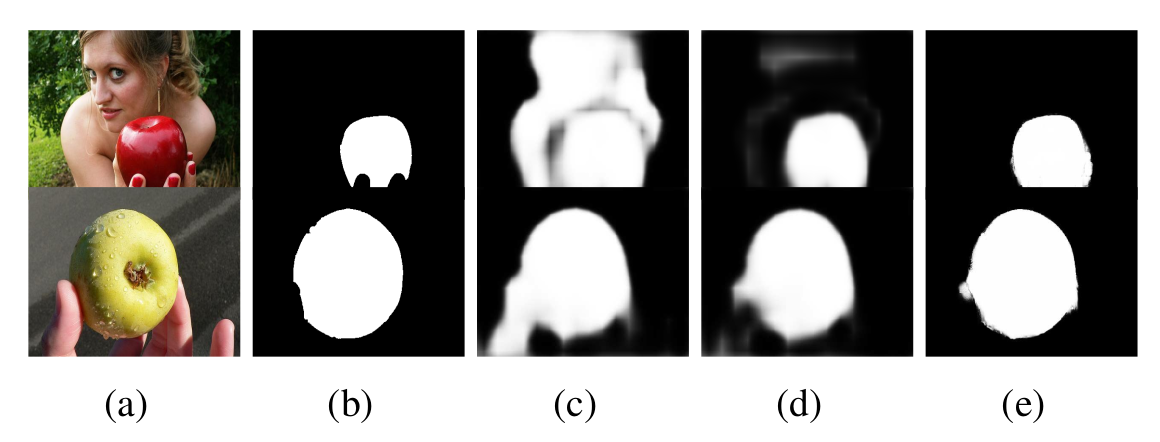
\includegraphics[width=1\textwidth]{steps.png}
		\caption{Różne mapy współwystępowania. (a) Obraz wejściowy; (b) Prawda; (c) Wyniki z sieci FCN bez wykorzystania maski; (d) FCN z wykorzystaniem maski; (e)  Efekt końcowy.}
		\label{step}
	\end{figure}

	\section{Opis}
	Metoda ta wykorzytuje hierarchiczne podejście do wykrywania współwystępowania. Algorytm składa się z dwóch głównych faz działania. W pierwszym kroku generowane są wstępne wyniki wykrywania współwystępowania za pomocą sieci w pełni splotowej wykorzystującej maskę (mask-guided fully convoluconal network - FCN). Architektura FCN opisana jest dokładnie w \cite{10.1109/TPAMI.2016.2572683}.	Podobne sieci sprawdzają się w problemach takich jak segmentacja oraz wykrywanie obiektów, ponieważ maska pozwala na zakodowanie istotnych informacji dotyczących przestrzeni. Pozwala to na wyuczenie się lepszych cech przez sieć splotową. W przypadku tej metody maska wykorzystywana jest do usunięcia tła w czasie uczenia sieci splotowej. Wynikowe mapy współwystępowania poprawiane są następnie z wykorzystanie techniki multi-scale label smoothing model.

	

	Do wykrywania współwystępowania wykorzystywana jest sieć mask-guided FCN. Splotowa część sieci składa się z dwóch kanałów przetwarzania. Do każdego z nich maska aplikowana w różnych warstwach. Wyniki z obu kanałów są następnie łączone oraz przesłane do warstwy odwrotnej do splotowej w celu wyznaczenia ostatecznych map współwystępowania.
	
	Maska użyta jest w celu poprawy działania sieci. Jest ona wyznaczana z wcześniej wyuczonej sieci VGG \cite{SimonyanZ14a}. Proces tworzenia maski zaprojektowany został tak, aby zmaksymalizować wariancję maski. Optymalizacja dokonana jest za pomocą algorytmu typu ADMM.

	W celu poprawy jakości map wynikowych użyta jest technika multi-scale label smoothing model. Model bierze pod uwagę gładkość zarówno pikseli, jak i superpikseli. Optymalizacja dokonana jest za pomocą algorytmu iteracyjnego.

	\begin{figure}[h!]
		\centering
		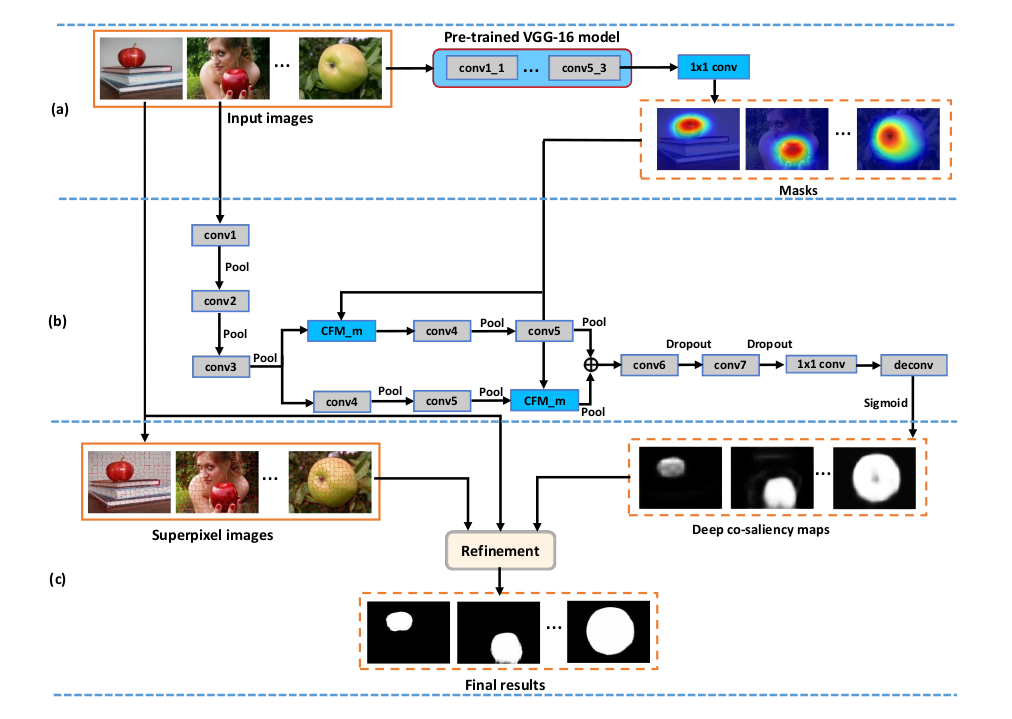
\includegraphics[width=1\textwidth]{fram.png}
		\caption{Zaproponowany przez autorów szkielet wykrywania współwystępowania. Krok (a) generuje maskę, która wyznacza obszary współwystępowania. Krok (b) zawiera sieć FCN, która po podziale na dwa kanały zostaje połączona z maskami (zaznaczonymi jako CFM\_m). Generuje ona głębokie mapy współwystępowania. Krok (c) zawiera poprawę wyników za pomocą multi-label smoothing model.}
		\label{fram}
	\end{figure}

	\section{Implementacja}
	TODO

	\addcontentsline{toc}{chapter}{Bibliografia}
	\bibliographystyle{acm}
	\bibliography{./bibliografia}
	
	
	% Nie sieć konwolucyjna, a SPOLOTOWA
	% Panoptic segmentation - zamiast superpiksele
	% Maski przede wszytskim

	
\end{document}
